\documentclass[useAMS,usenatbib]{mn2e}
\usepackage{float}
\usepackage{amsmath}
\usepackage{amssymb}
\usepackage{graphics}
\usepackage{graphicx}
\usepackage{epsfig} 
\usepackage{hyperref}
\def\be{\begin{equation}}
\def\ee{\end{equation}}
\def\ba{\begin{eqnarray}}
\def\ea{\end{eqnarray}}

% To highlight comments
\usepackage{color}
\definecolor{red}{rgb}{1,0.0,0.0}
\newcommand{\red}{\color{red}}
\definecolor{blue}{rgb}{0.1,0.3,0.9}
\newcommand{\blue}{\color{blue}}

\usepackage[normalem]{ulem}
\definecolor{darkgreen}{rgb}{0.0,0.5,0.0}

\newcommand{\documentname}{paper~}
\newcommand{\LCDM}{$\Lambda$CDM~}
\newcommand{\beq}{\begin{eqnarray}} 
\newcommand{\eeq}{\end{eqnarray}} 
\newcommand{\zz}{$z\sim 3$}

\newcommand{\apj}{ApJ} 
\newcommand{\apjs}{ApJS} 
\newcommand{\apjl}{ApJL} 
\newcommand{\aj}{AJ} 
\newcommand{\mnras}{MNRAS} 
\newcommand{\mnrassub}{MNRAS accepted} 
\newcommand{\aap}{A\&A} 
\newcommand{\aaps}{A\&AS} 
\newcommand{\araa}{ARA\&A} 
\newcommand{\nat}{Nature} 
\newcommand{\physrep}{PhR}
\newcommand{\pasp}{PASP}   
\newcommand{\pasj}{PASJ}   
\newcommand{\avg}[1]{\langle{#1}\rangle} 
\newcommand{\ly}{{\ifmmode{{\rm Ly}\alpha}\else{Ly$\alpha$}\fi}}
\newcommand{\hMpc}{{\ifmmode{h^{-1}{\rm Mpc}}\else{$h^{-1}$Mpc }\fi}} 
\newcommand{\hGpc}{{\ifmmode{h^{-1}{\rm Gpc}}\else{$h^{-1}$Gpc }\fi}} 
\newcommand{\hmpc}{{\ifmmode{h^{-1}{\rm Mpc}}\else{$h^{-1}$Mpc }\fi}} 
\newcommand{\hkpc}{{\ifmmode{h^{-1}{\rm kpc}}\else{$h^{-1}$kpc }\fi}}
\newcommand{\hMsun}{{\ifmmode{h^{-1}{\rm
        {M_{\odot}}}}\else{$h^{-1}{\rm{M_{\odot}}}$~}\fi}}  
\newcommand{\hmsun}{{\ifmmode{h^{-1}{\rm
        {M_{\odot}}}}\else{$h^{-1}{\rm{M_{\odot}}}$}\fi}}  
\newcommand{\Msun}{{\ifmmode{{\rm {M_{\odot}}}}\else{${\rm{M_{\odot}}}$}\fi}} 
\newcommand{\msun}{{\ifmmode{{\rm {M_{\odot}}}}\else{${\rm{M_{\odot}}}$}\fi}} 
\newcommand{\lya}{{Lyman$\alpha$~}}
\newcommand{\clara}{{\texttt{CLARA}}~}
\newcommand{\rand}{{\ifmmode{{\mathcal{R}}}\else{${\mathcal{R}}$ }\fi}} 
\newcommand{\hs}{{\hspace{1mm}}}
\newcommand{\muavg}{\vert\langle\cos\theta\rangle\vert}
% definition to produce a "less than or similar to" symbol
\def\lsim{~\rlap{$<$}{\lower 1.0ex\hbox{$\sim$}}}

% definition to produce a "greater than or similar to" symbol

% definition to produce a "greater than or similar to" symbol
\def\gsim{~\rlap{$>$}{\lower 1.0ex\hbox{$\sim$}}}

\begin{document}

\title[New approach to Halo concentrations]{A new method to estimate
  dark matter halo concentrations}
\author[Poveda \& Forero-Romero]{
\parbox[t]{\textwidth}{\raggedright
  Christian Poveda$^{1}$ \&
  Jaime E. Forero-Romero$^{1}$
}
\vspace*{6pt}\\
$^{1}$Departamento de F\'{i}sica, Universidad de los Andes, Cra. 1
No. 18A-10, Edificio Ip, Bogot\'a, Colombia\\
}
\maketitle

\begin{abstract}
asd
\end{abstract}
\begin{keywords}
methods: numerical, galaxies: haloes, cosmology: theory, dark
matter
\end{keywords}


\section{Introduction}
\label{sec:introduction}
In the concordance cosmology paradigm the the matter content of the
Universe are dominated by dark matter which behaves as a collisionless
fluid under the influence of gravity. In the last three decades
numerical experiments have made possible the simulation of large
volumes of a Universe dominated by dark matter. 

One of the most striking results of these simulations is that dark
matter clumps on galactic scales follows a universal density profile
which in a first approximation is spherical symmetric and only
dependent on the radial coordinate. These profiles seem to be
universal; independent of the cosmological parameters and self-similar
for different spatial scapes after an addecuate re-scaling is
appplied.

One the most commong parameterization of this density is known as the
Navarro-Frenk-White (NFW) profile \citep{NFW}. This profile is a
double power law in radius, where the transition between the two
happens at the so-called scale radius $r_s$. The ratio between the
scale radius and the virial radius of the halo $R_v$ is known as the
concentration $c=R_V/r_s$, a quantity that has been found to be
correlated with the halo mass.  

The relationship between halo mass and concentration is in principle
accesible to observations and provides a potential test of LCDM on
galactic scales. With this promise a great deal of effort has been
invested in calibrating this relationship with simulations but also
finding the best possible way to constraint it with observations.

From the computational point of view there are two main methods to
estimate the concetration parameter of a dark matter halo in a N-body
simulation. The first method takes the particles comprosing the halos
and bins them in logarithmic radii to estimate the density in each
bin, then it proceeds with a fit of this density estimation as a
function of radius. A second method uses an analytical property of the
NFW that related the maximum of the ratio of the circular velocity to
the virial velocity. In this method at each particle radius this ratio
is estimated to find the maximum value for this ratio; this value is
used to find the roots of an equation which represent the
concentration parameter. 

The first method although is straightforward to apply has two main
disadvantages. First of all it requires a large number of particles in
order to have a proper density estimate in each bin. For a very low
number of particles is hard to define a large number of bins to
proceed with the fit. The second problem is that, as in any process
involving data binning, there is not an way to estimate the optimal
bin size, which in turn can affect the results of the fit.

The second method solves the two problems mentioned above. It works
with low particles numbers and does not involve data binning. However,
it effectively takes into account a single data point and discards the
behaviour of the ratio $V_{cirv}/V_{vir}$ below and above its
maxima. 

In this paper we propose a new method to estimate the dark matter halo
concentration from N-body simulation results. This method has two
advantages with respect to the methods mentioned above. First, it does
not involve data binning. Second, it does not throw away data
points. Third, it allows for an straightforward estimation of the
uncertainties in the concentration parameter. 

Our method consists in building the cumulative mass profile from the
particle data in the N-body simulation to find the best possible
concentration value using a Markov Chain Monte Carlo methodology by
comparing the data against the analytical expectation.

This paper is structured as follows. In Section \ref{sec:basics} we
review the basic properties of the NFW density profile and define the
basic notation for the rest of the paper. Next in Section
\ref{sec:method} we present our new method to estimate the halo
concentration, payin special attention to the bayesian framework to
find the most probable value and its uncertaintt. In Section
\ref{sec:halo_sample} we demonstrate the power of our method with two
different halo samples; the first one generated under controlled
conditions and the second taken from a cosmological N-body
simulation. Next in \ref{sec:discussion} we discuss these results by
comparing them against other methods to estimate the concentration and
comment on the consequences for the concentration-mass
relationship. We present our conclusions in Section \ref{sec:conclusions}.









\section{Basic properties of the NFW density profile}
\label{sec:basics}

The Navarro-Frenk-White density profile can be written as

\begin{equation}
\rho(r) = \frac{\rho_c\delta_c}{r/r_s(1+r/r_s)^2}, 
\end{equation}
%
where $\rho_c\equiv 3H^2/8\pi G$ is the Universe critical density,
$\delta_c$ is the halo dimensionless characteristic density and $r_s$
is known as the scale radius, the radius that marks the transition
between the two power law behaviour in the $\rho\propto r^{-1}$ for
$r<r_s$ and $\rho\propto r^{-3}$ for  $r>r_s$.  

We define the virial radius of a halo, $r_v$, as the boundary of the
spherical volume that encloses an average density of $\Delta_h$ times
the average density of the Universe. The corresponding mass $M_{v}$,
the virial mass, can be written as $M_{v} =
\frac{4\pi}{3}\bar{\rho}\Delta_h r_v^3$. 


\subsection{Integrated Mass}
From these definitions we can compute the total mass enclosed inside a
radius $r$:
\begin{equation}
M(<r) = 4\pi\rho_c\delta_c  r_s^3\left[\ln \left
  (\frac{r_s+r}{r}\right) - \frac{r}{r_s+r}\right].
\end{equation}
 
We can now express the same quantity in terms of dimensionless the
variables $x\equiv r/r_v$ and $m\equiv M(<r)/M_v$,
%
\begin{equation}
m(<x) =
\frac{1}{A}\left[\ln\left(1+xc\right)-\left(\frac{xc}{xc+1}\right)\right],
\label{eq:profile}
\end{equation}
%
where 
%
\begin{equation}
A=\left[\ln\left(1+c\right)-\left(\frac{c}{c+1}\right)\right],
\end{equation}
%
and the parameter $c$ is known as the concentration $c\equiv r_v/r_s$.

The most interesting feature of Eq. (\ref{eq:profile}) is that the
concentration is the only free parameter to describe the density
profile. In Figure \ref{fig:profiles} we show $m(<x)$ as 
a function of $x$ for different values of the concentration in the range
$1\leq c \leq 20$.  

\begin{figure}
\begin{center}
  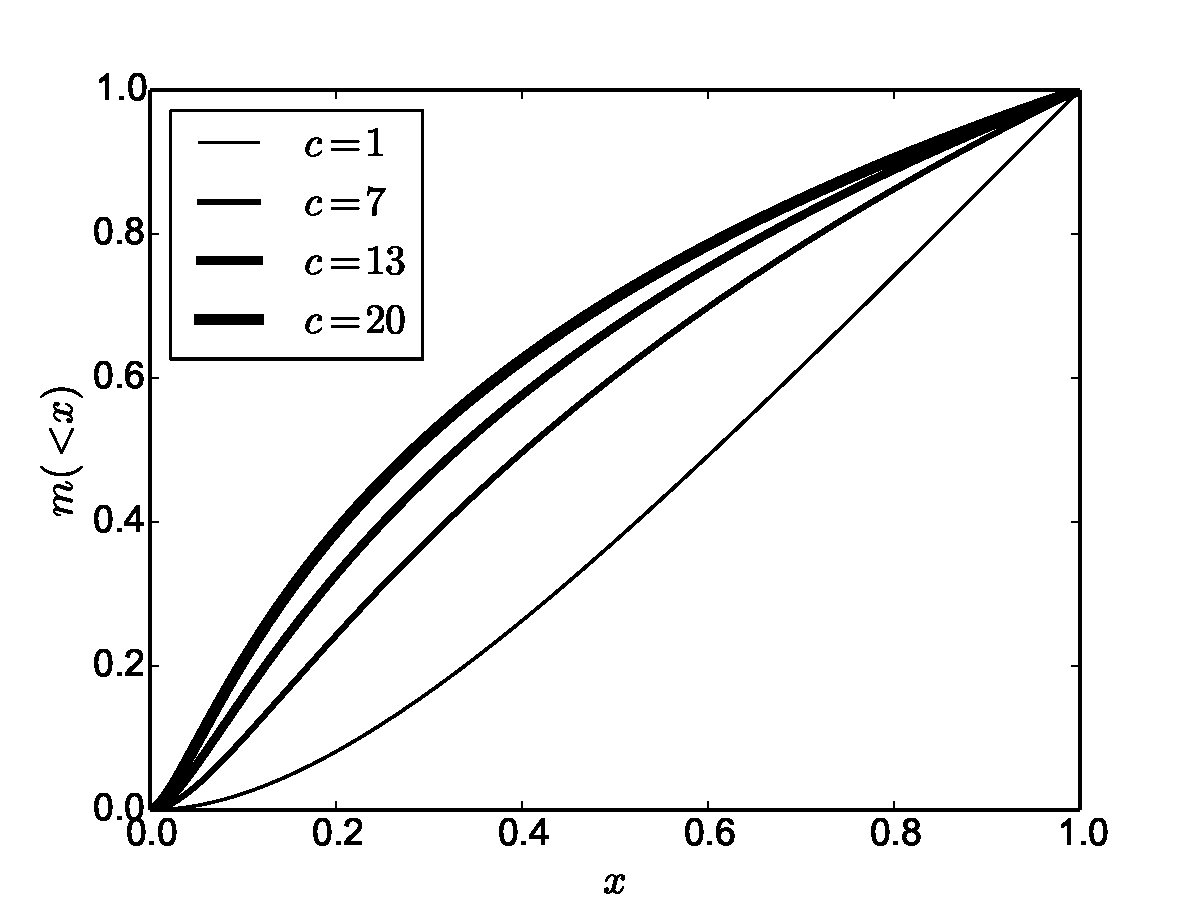
\includegraphics[width=0.48\textwidth]{nfw_normalized.pdf}
\end{center}
\caption{Dimensionless mass profiles as a function of the
  dimensionless radius for different concentration values.
    \label{fig:profiles}}
\end{figure}

\subsection{Circular velocity}

It is also customary to express the mass of the halo inte terms of the
circular velocity $V_{c}=\sqrt{GM(<r)/r}$. From this we can
define a new dimensionless circular velocity $v(<x)\equiv
V_{c}(<r)/V_{c}(<r_v)$, using the result in Equation \ref{eq:profile}
to have:

\begin{equation}
v(<x)=\sqrt{\frac{1}{A}\left[\frac{\ln\left(1+xc\right)}{x}-\frac{c}{xc+1}\right]},
\end{equation}

\begin{figure}
\begin{center}
  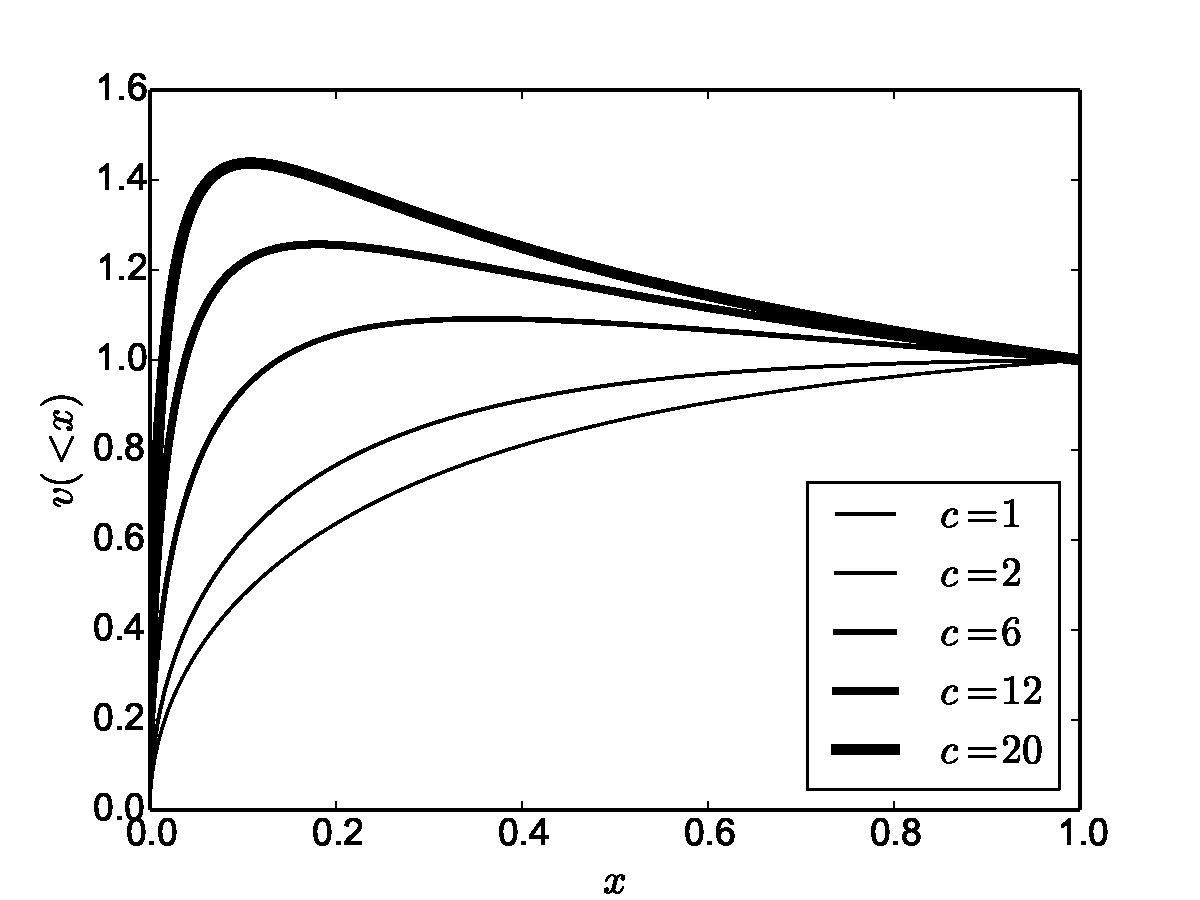
\includegraphics[width=0.48\textwidth]{vel_normalized.pdf}
\end{center}
\caption{Dimensionless velocity profiles as a function of the
  dimensionless radius for different concentration values.
    \label{fig:velocity}}
\end{figure}

In Figure \ref{fig:velocity} we show the circular velocity profile for the same
concentrations as in Figure \ref{fig:profiles}.

\section{A new Approach to Halo Fitting}
\label{sec:method}


We estimate the concentration parameter by fitting the
integrated mass profile described in Equation
(\ref{eq:profile}). First we define the center of the halo to be  at
the position of the particle with the lowest gravitational
potential. 



We construct the integrated mass profile by ranking the particles by
their increasing distance to the center of the halo. Once they are ranked,
the total mass at a radius $r_i$, increases by $m_p$, where $r_i$ is
the position of the $i$-th particle and $m_p$ is the mass of the
computational particle.  In this process we discard the
particle at the center.  


We stop the construction of the integrated mass profile once we arrive
at an average density of $\Delta_h\bar{\rho}$, with $\Delta_h=740$,
roughly corresponding to 200 times the critical density. This radius marks the
virial radius and the virial mass. We divide the total mass enclosed
mass $M_i$ and the radii $r_i$ by these values to obtain the
dimensionless variables $x_i$ and $m_i$. 

Using these new variables we define the following $\chi^2$ function

\begin{equation}
\chi^2(c) = \sum_{i}[\log m_i - \log m(< x_i;c)]^2, 
\end{equation}
%
where $m(<x_i;c)$ corresponds to the values in Eq.(\ref{eq:profile}) at
$x=x_i$ for a given value of the concentration parameter $c$. 

We sample the likelihood function distribution defined by ${\cal
  L}(c)=\exp(-\chi^2(c)/2)$ with a Metropolos-Hastings algorithms to
find the optimum value of $c$ and its  associated uncertainty
$\sigma_c$.  


{\bf Cuantos pasos usa la cadena? (50000) De cuanto es el sigma en
los saltos de c en lca cadena? (0.029)

Falta alguna figura que muestre resultados de la -log likelihood para
algunos casos representativos.
}



\section{Results}
\label{sec:results}

We apply our method to two different halo samples. The first one is a
mock sample to test the algorithm and asses the impact of the number
of computational particles on the concentration values. The second
sample comes from a publicly available N-body cosmological
simulation. These results for these sample can be then compared
against other methods to find the concentration and feed the
discussion about the implications of our method.

\subsection{Mock Halos}

First, we test our method using mock halos with known values for the
concentration. The method we use to generate the halos is based on the integrated
mass profile. Given the number of particles $n$ and the concentration
$c$ we define the mass element as $\delta m = 1/n$ (this corresponds
to the mass of each particle such that the total mass is one). Then
for each number $k$ from $1$ to $n$ we find the value of $r$ such that
the difference 
%
\begin{equation}
m(<r;c)-k \cdot \delta m 
\end{equation}
%
is zero using Ridders' method. This value of $r$ is the radius of
the $k$th particle of the generated halo, then polar and azimuthal
angles $\theta$ and $\phi$ are randomly generated. Finally these three
coordinates are transformed into cartesian coordinates
$(r,\theta,\phi) \rightarrow (x,y,z)$. This process is repeated $n$
times in order to generate the $x,y,z$ coordinates for each particle. 
 


We generate $100$ mock halos with concentration values randomly
placed in the range $1<c<20$. Each one of the halos is generated with
four different total particle numbers: $20$, $200$, $2000$ and
$20000$. This gives us a total of $500$ halos. 


\begin{figure}
\begin{center}
  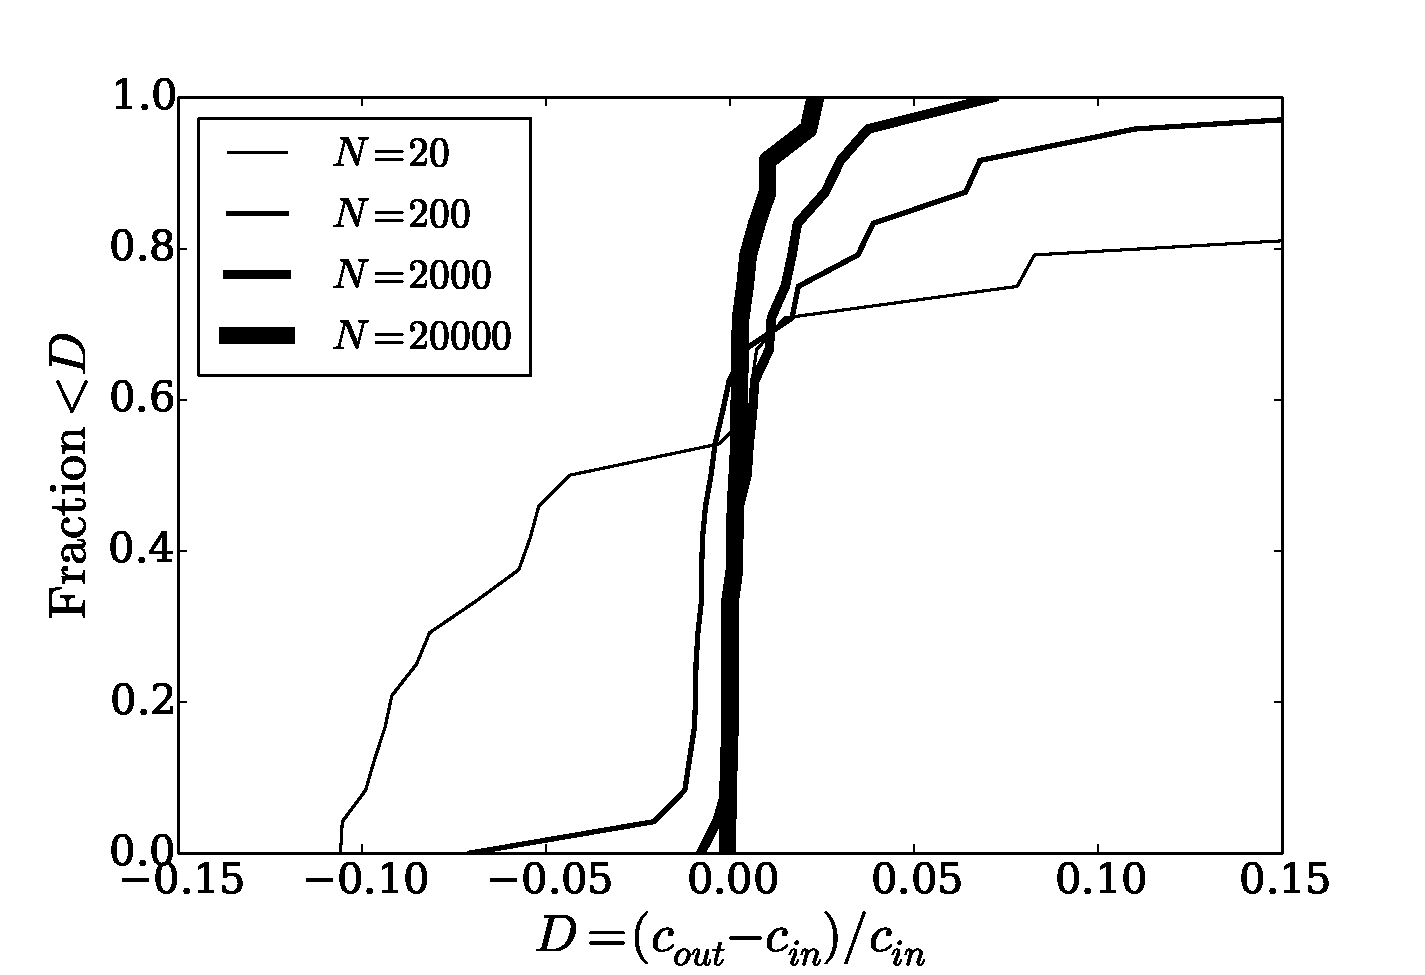
\includegraphics[width=0.48\textwidth]{percentual_diff.pdf}
\end{center}
\caption{Cumulative distribution of the fractional difference between
  the input concentration in the mock halo generator, $c_{in}$ and the
  measurement by our MCMC code, $c_{out}$. Each curve corresponds to
  halos generated with a different number of particles, $N$.
    \label{fig:results_mocks}}
\end{figure}


In Figure \ref{fig:results_mocks} we show the integrated distribution
percentual difference between the concentration measured with our
fitting method $c_{out}$ in comparison with the concentration used to
generate the mock halos, $c_{in}$, $D=(c_{in}-c_{out})/c_{in}$. Then we can see that as the number of particles increases, the curve becomes more pronounced at 0. Showing that for most of the halos $c_{in}$ is very similar to $c_{out}$.




\subsection{Simulation Data}
\label{sec:data}

We use data from the MultiDark cosmological volume. This simulation
follows the non-linear evolution of a dark matter density field
sampled with $2048^3$ particles over a cubic box of $1000$ \hMpc on a
side. The data is publicly available, more details about the structure
of the database and the simulations can be found in
\citep{2013AN....334..691R}. 

We select a sample of halos in a cubic sub-volumne of $100$ \hMpc on a
side centered on the most massive halo in the simulation at
$z=0$\footnote{This corresponds to the \texttt{miniMDR1} database in
  the MultiDark webpage}. We select first all the halos at $z=0$
detected with a Friends-of-Friends (FoF) algorithm with masses in the
interval $10^{11}\leq M_{\rm FoF}/\hMsun \leq 10^{15}$. The FoF
algorithm ran with a linking length of $0.17$ times the average
interparticle distance. This choice translates into an overdensity
$\Delta_h\sim 400-700$ that is dependent on the halo concentration
\citep{More2011}.

For each selected halo with the previous procedure we select from the database
all the particles that belong to it. From the particles we follow the
procedure spelled out in Section \ref{sec:method} with $\Delta_h=740$
(corresponding to $200$ times the critical density) to find the
halo concentration. Finally, we store the values obtained for the
virial radius, virial mass and concentration. 



\section{Discussion}
\label{sec:discussion}


\subsection{Comparison against other methods}
\label{sec:comparison}
We compared this method against two methods: The first one consists in
using shells for estimating the density in function of the radius and
using the same MCMC method for fitting and the second one consists in
using the circular velocity $V(r)=\sqrt{GM(<r)/r}$ and the relation
for the NFW profile 
\begin{equation}
\frac{V_{max}}{V(r_{v})} = \sqrt{\frac{0.216c}{M(r_{v};c)}}
\end{equation}
Where $V_{max}$ is the maximum velocity, to find the value of the concentration. We tested the three methods using the same data from the Mock Halos test. In order to see the accuracy of each method depending on the number of particles we define 

\begin{equation}
\xi(n)=\frac{1}{\left|{\cal{H}}_n\right|}\sum_{{\cal{H}}_n}\left|\frac{c_{org}-c_{obt}}{c_{org}}\right|
\end{equation}

Where ${\cal{H}}_n$ corresponds to the set of haloes with $n$ particles, $c_{org}$ and $c_{obt}$ are the original and obtained concentrations respectively for each halo in ${\cal{H}}_n$ and $\left|{\cal{H}}_n\right|$ the number of haloes in ${\cal{H}}_n$. Then we calculate $\xi$ for each number of particles (20, 200, 2000 and 20000).

\begin{figure}
\begin{center}
  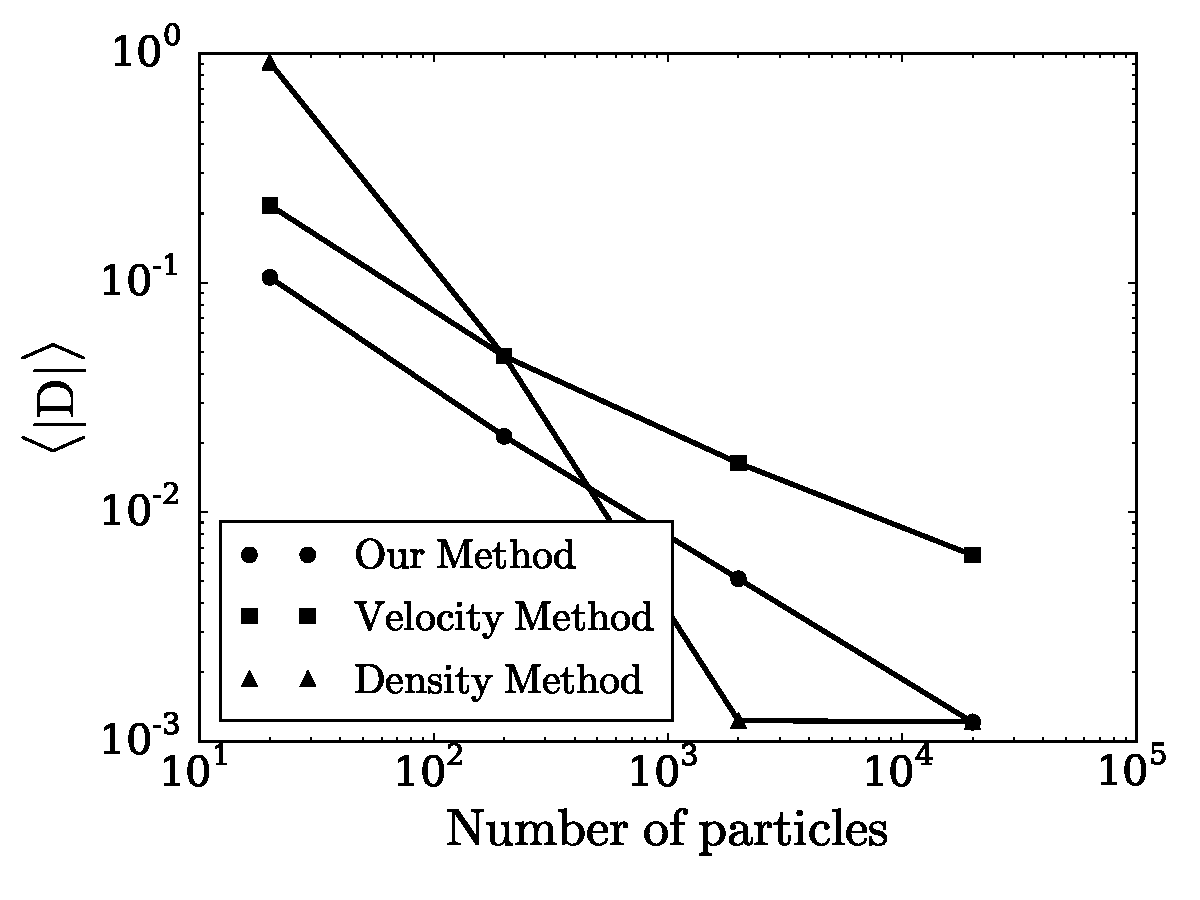
\includegraphics[width=0.48\textwidth]{error.pdf}
\end{center}
\caption{Relative error against number of particles
    \label{fig:error}}
\end{figure}

In Figure \ref{fig:error} we plotted $\xi$ for the three methods. We consider that $\xi$ is a good estimate because it is standardized, giving equal weight to all errors regardless of the magnitude of the concentrations or the number of halos. On the other hand we have that $\xi$ decreases quite fast with the number of particles for our method and is more precise in any case that the other methods. As mentioned in FIXME \textit{``for a large fraction of halos, and for the most massive in particular, the NFW functional does not Represent a good fit to the density profile."} This fact could explain why $\xi$ increases with the number of particles for the density method.

\begin{figure*}
\begin{center}
  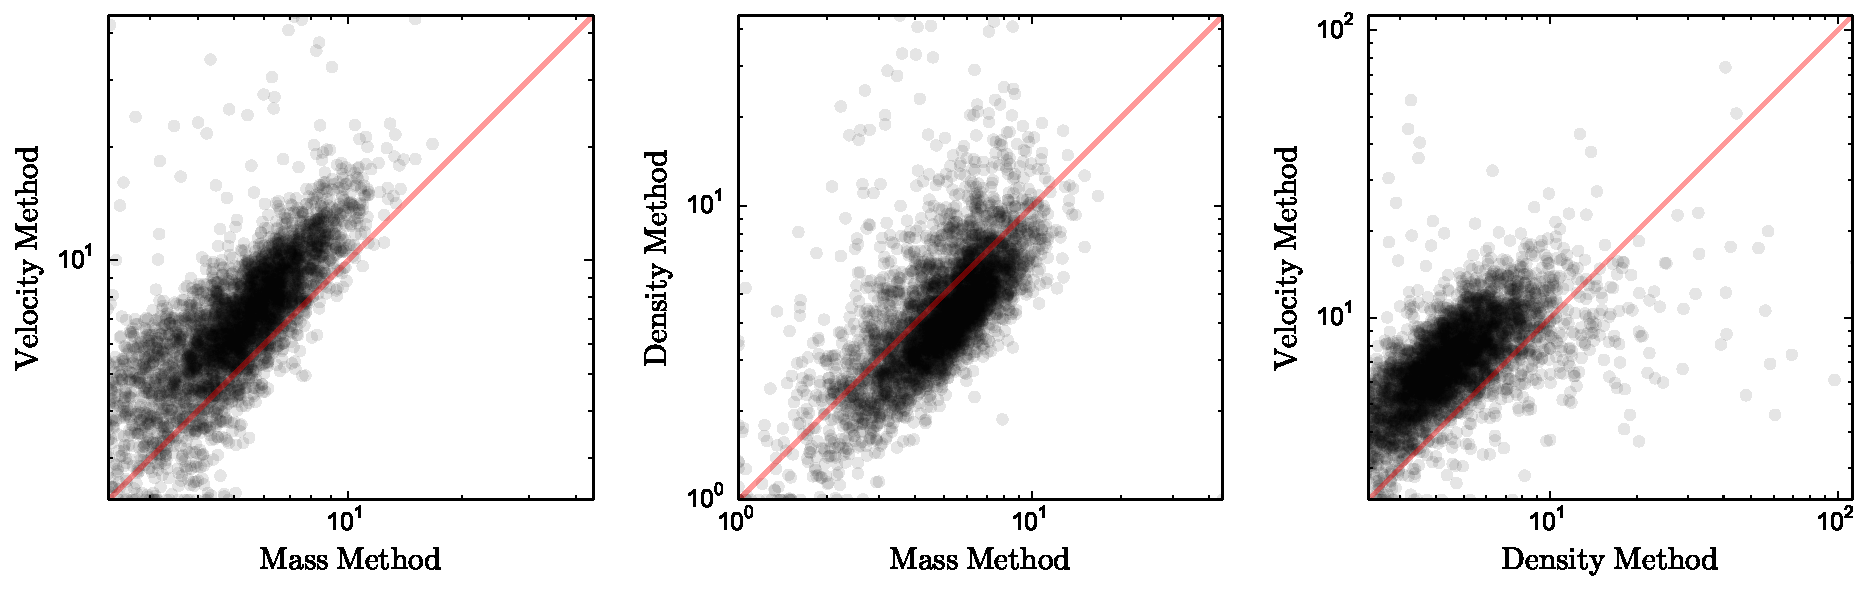
\includegraphics[width=0.99\textwidth]{mass-density-velocity.pdf}
\end{center}
\caption{Comparison between the obtained concentrations by the three methods
    \label{fig:mdv}}
\end{figure*}

We also used these three methods to obtain the concentration for each halo in miniMDR1 and compared the results. As can be seen in Figure \ref{fig:mdv} the three methods show mutually consistent results. However it can be inferred that the concentration values ​​obtained by the method of circular velocity are higher than those obtained by our method, and also the values ​​obtained by the density method are generally below the results of our method.

Running another test with halos whose concentrations vary as a normal
distribution of variance ${\sigma}^2$ we found that the concentrations
obtained by the method of circular velocity are a 35\% greater than
the ones obtained by the density method. However the concentrations
obtained by the velocity method are barey higher (around 2\% or 3\%)
than the ones obtained by our method. We did not find any significant
variation in the concentration values obtained by any method by
changing ${\sigma}^2$ in contrast with FIXME. 




\subsection{Impact on the mass-concentration relationship}
Aditionally we compared those three methods plotting the concentration as a function of the number of particles of each halo 

\begin{figure}
\begin{center}
  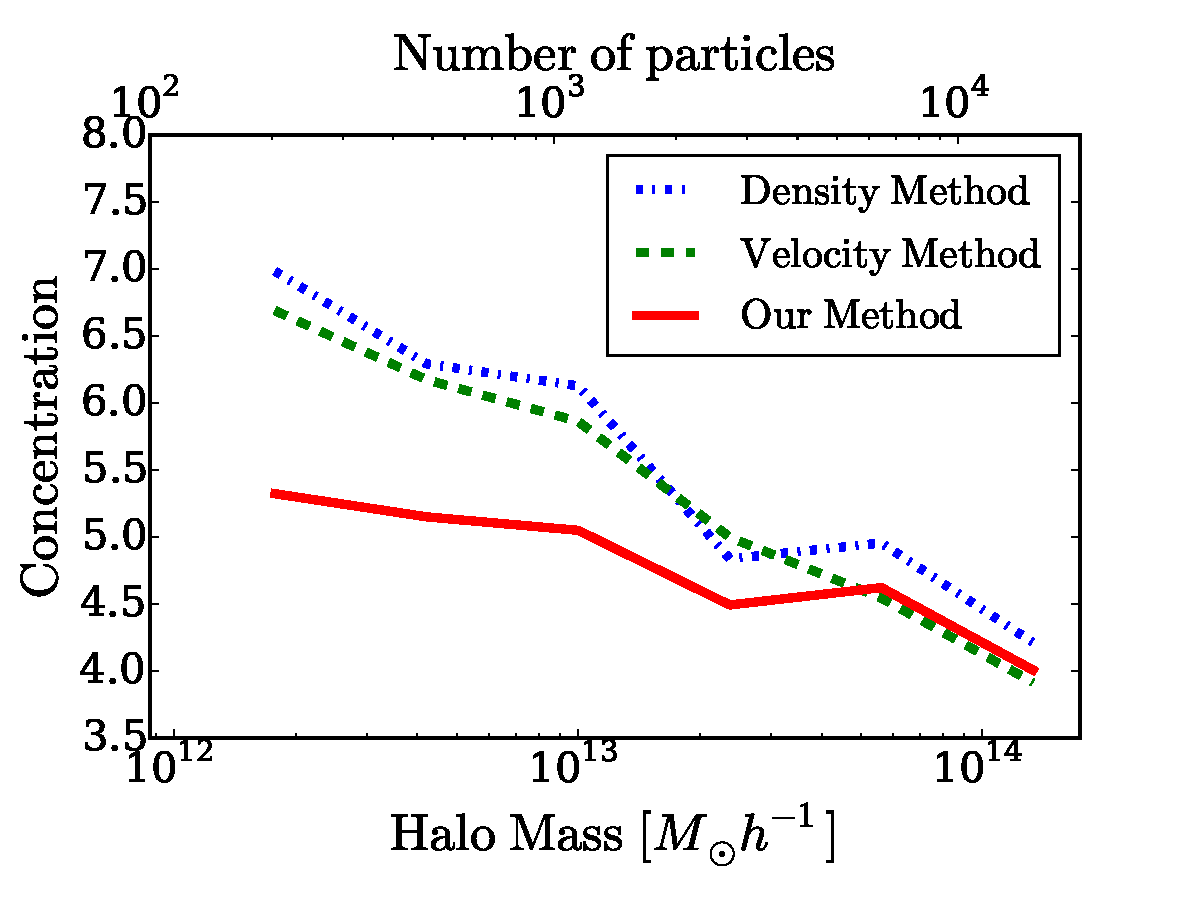
\includegraphics[width=0.48\textwidth]{concentration.pdf}
\end{center}
\caption{Concentration against number of particles
    \label{fig:concentrations}}
\end{figure}

The bold lines in Figure \ref{fig:concentrations} corresponds to the median and the thinner lines corresponds to the quartiles. Showing that our method has values ​​ranging from those obtained from the other two methods.Also we can see that the concentration obtained by the velocity method is higher than that obtained by the density method, this fact is consistent with FIXME.
\subsection{Implication for comparisons against observations}
FIXME: Ask Jaime

\section{Conclusions}
\label{sec:conclusions}
FIXME: Ask Jaime

\bibliographystyle{mn2e}
\bibliography{references}

\verb"http://adsabs.harvard.edu/abs/2014ApJ...795..163U"
\verb"http://adsabs.harvard.edu/abs/2012ApJS..199...25P" Figura 3!
\end{document}
